\documentclass[11pt,a4paper]{article}

% Packages
\usepackage[utf8]{inputenc}
\usepackage[T1]{fontenc}
\usepackage{amsmath,amssymb}
\usepackage{graphicx}
\usepackage{booktabs}
\usepackage{array}
\usepackage{tikz}
\usetikzlibrary{shapes,arrows,positioning,fit,calc,backgrounds,decorations.pathreplacing,arrows.meta}
\usepackage{xcolor}
\usepackage[hidelinks]{hyperref}
\usepackage{geometry}
\geometry{margin=0.9in}
\usepackage{float}
\usepackage{multirow}

% Colors
\definecolor{globalcolor}{RGB}{100, 149, 237}
\definecolor{statecolor}{RGB}{144, 238, 144}
\definecolor{actorcolor}{RGB}{255, 182, 108}
\definecolor{dynamicscolor}{RGB}{255, 160, 160}
\definecolor{ballcolor}{RGB}{221, 160, 221}
\definecolor{querycolor}{RGB}{255, 255, 150}
\definecolor{edgecolor}{RGB}{150, 150, 150}

\title{Cricket Ball Prediction Model V2:\\Unified Heterogeneous Graph Architecture}
\author{Architecture Documentation}
\date{\today}

\begin{document}

\maketitle

\begin{abstract}
This document describes Version 2 of the cricket ball prediction model. The key innovation is representing \textbf{all information as a single heterogeneous graph}, eliminating the separation between spatial and temporal processing. This enables full innings history while maintaining computational efficiency.
\end{abstract}

\tableofcontents
\newpage

%==========================================
\section{Overview}
%==========================================

\subsection{The Core Idea}

Instead of separate spatial and temporal streams, \textbf{everything becomes one heterogeneous graph}.

\begin{figure}[H]
\centering
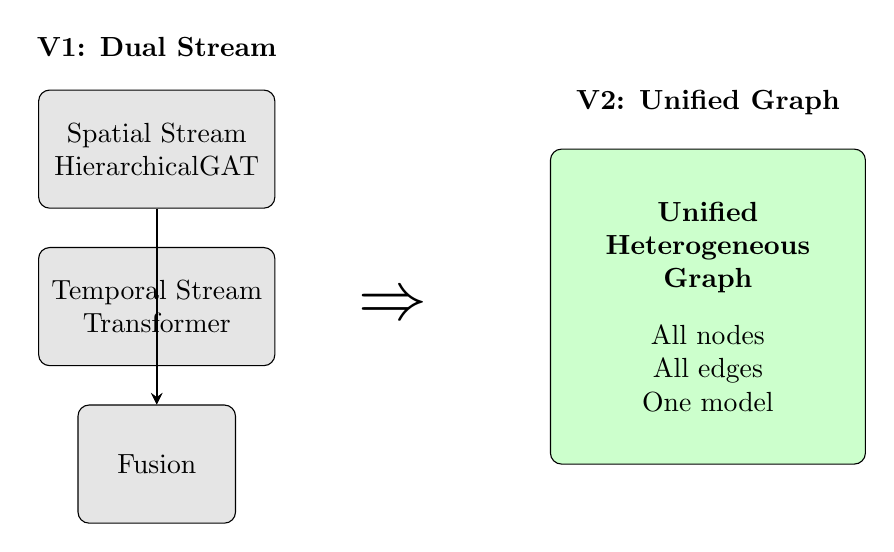
\begin{tikzpicture}[
    oldbox/.style={rectangle, draw, rounded corners, minimum width=3cm, minimum height=1.5cm, align=center, fill=gray!20},
    newbox/.style={rectangle, draw, rounded corners, minimum width=4cm, minimum height=2cm, align=center, fill=green!20},
    arrow/.style={->, thick, >=stealth}
]
    % V1
    \node[oldbox] (spatial) at (-3, 2) {Spatial Stream\\HierarchicalGAT};
    \node[oldbox] (temporal) at (-3, 0) {Temporal Stream\\Transformer};
    \node[oldbox, minimum width=2cm] (fusion) at (-3, -2) {Fusion};

    \draw[arrow] (spatial) -- (fusion);
    \draw[arrow] (temporal) -- (fusion);

    \node[above=0.3cm of spatial] {\textbf{V1: Dual Stream}};

    % Arrow
    \node at (0, 0) {\Huge $\Rightarrow$};

    % V2
    \node[newbox, minimum height=4cm] (unified) at (4, 0) {
        \textbf{Unified}\\
        \textbf{Heterogeneous}\\
        \textbf{Graph}\\[0.3cm]
        All nodes\\All edges\\One model
    };

    \node[above=0.3cm of unified] {\textbf{V2: Unified Graph}};
\end{tikzpicture}
\caption{Architecture evolution from V1 (dual stream) to V2 (unified graph)}
\end{figure}

\subsection{Why This Matters}

\begin{table}[H]
\centering
\begin{tabular}{lll}
\toprule
Aspect & V1 (Dual Stream) & V2 (Unified Graph) \\
\midrule
History length & Fixed 24 balls & Full innings \\
Complexity & O(n²) attention & O(edges) \\
Same-bowler patterns & Soft attention bias & Explicit edges \\
Information flow & Separate then fuse & Unified message passing \\
Framework & Mixed PyTorch/PyG & Full PyTorch Geometric \\
\bottomrule
\end{tabular}
\end{table}

\newpage
%==========================================
\section{The Unified Graph Structure}
%==========================================

\subsection{Node Types}

The graph contains \textbf{6 node type categories}:

\begin{figure}[H]
\centering
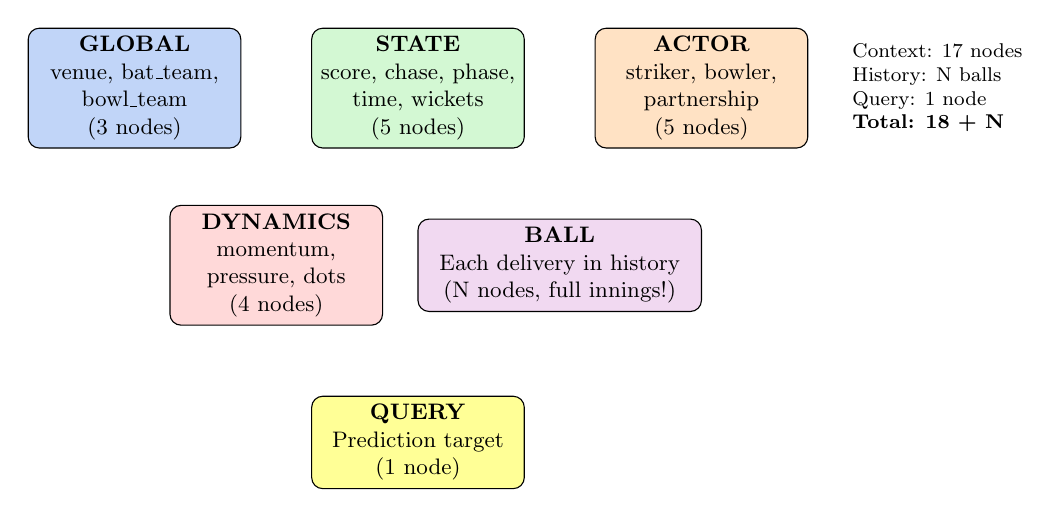
\begin{tikzpicture}[
    nodetype/.style={rectangle, draw, rounded corners, minimum width=3cm, minimum height=1.2cm, align=center, font=\small},
    scale=0.9, transform shape
]
    % Global
    \node[nodetype, fill=globalcolor!40] (global) at (-4, 4) {
        \textbf{GLOBAL}\\
        venue, bat\_team,\\bowl\_team\\(3 nodes)
    };

    % State
    \node[nodetype, fill=statecolor!40] (state) at (0, 4) {
        \textbf{STATE}\\
        score, chase, phase,\\time, wickets\\(5 nodes)
    };

    % Actor
    \node[nodetype, fill=actorcolor!40] (actor) at (4, 4) {
        \textbf{ACTOR}\\
        striker, bowler,\\partnership\\(5 nodes)
    };

    % Dynamics
    \node[nodetype, fill=dynamicscolor!40] (dynamics) at (-2, 1.5) {
        \textbf{DYNAMICS}\\
        momentum,\\pressure, dots\\(4 nodes)
    };

    % Ball
    \node[nodetype, fill=ballcolor!40, minimum width=4cm] (ball) at (2, 1.5) {
        \textbf{BALL}\\
        Each delivery in history\\(N nodes, full innings!)
    };

    % Query
    \node[nodetype, fill=querycolor, minimum width=3cm] (query) at (0, -1) {
        \textbf{QUERY}\\
        Prediction target\\(1 node)
    };

    % Counts
    \node[right=0.5cm of actor, align=left, font=\footnotesize] {
        Context: 17 nodes\\
        History: N balls\\
        Query: 1 node\\
        \textbf{Total: 18 + N}
    };
\end{tikzpicture}
\caption{Six node type categories in the unified graph}
\end{figure}

\subsection{Edge Types}

\begin{figure}[H]
\centering
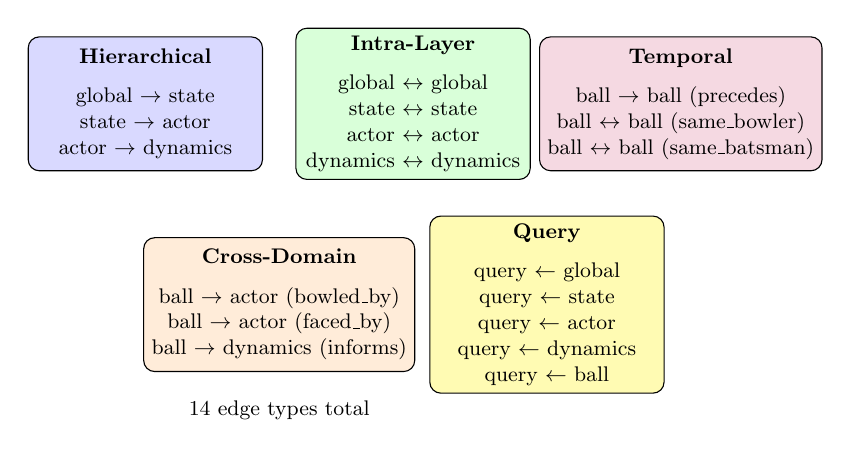
\begin{tikzpicture}[
    box/.style={rectangle, draw, rounded corners, minimum width=3.5cm, minimum height=2cm, align=center, font=\small},
    scale=0.85, transform shape
]
    % Hierarchical
    \node[box, fill=blue!15] (hier) at (-4, 3) {
        \textbf{Hierarchical}\\[0.2cm]
        global $\to$ state\\
        state $\to$ actor\\
        actor $\to$ dynamics
    };

    % Intra-layer
    \node[box, fill=green!15] (intra) at (0, 3) {
        \textbf{Intra-Layer}\\[0.2cm]
        global $\leftrightarrow$ global\\
        state $\leftrightarrow$ state\\
        actor $\leftrightarrow$ actor\\
        dynamics $\leftrightarrow$ dynamics
    };

    % Temporal
    \node[box, fill=purple!15] (temporal) at (4, 3) {
        \textbf{Temporal}\\[0.2cm]
        ball $\to$ ball (precedes)\\
        ball $\leftrightarrow$ ball (same\_bowler)\\
        ball $\leftrightarrow$ ball (same\_batsman)
    };

    % Cross-domain
    \node[box, fill=orange!15] (cross) at (-2, 0) {
        \textbf{Cross-Domain}\\[0.2cm]
        ball $\to$ actor (bowled\_by)\\
        ball $\to$ actor (faced\_by)\\
        ball $\to$ dynamics (informs)
    };

    % Query
    \node[box, fill=yellow!30] (query) at (2, 0) {
        \textbf{Query}\\[0.2cm]
        query $\leftarrow$ global\\
        query $\leftarrow$ state\\
        query $\leftarrow$ actor\\
        query $\leftarrow$ dynamics\\
        query $\leftarrow$ ball
    };

    \node[below=0.3cm of cross, font=\small] {14 edge types total};
\end{tikzpicture}
\caption{Edge type categories encoding different relationships}
\end{figure}

\newpage
%==========================================
\section{Full Graph Visualization}
%==========================================

\begin{figure}[H]
\centering
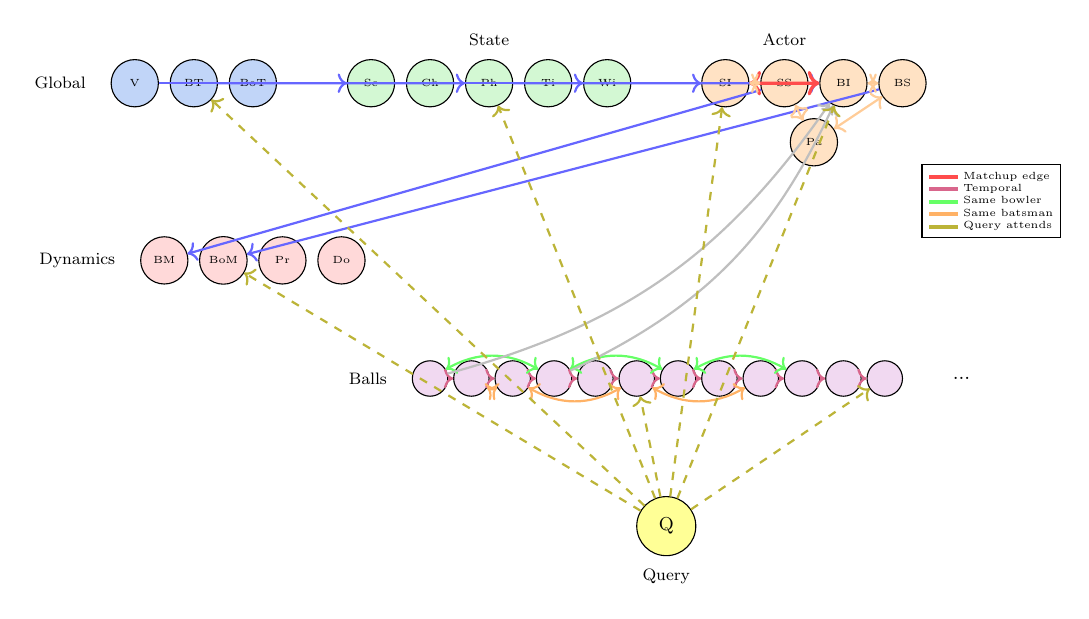
\begin{tikzpicture}[
    gnode/.style={circle, draw, fill=globalcolor!40, minimum size=0.8cm, font=\tiny},
    snode/.style={circle, draw, fill=statecolor!40, minimum size=0.8cm, font=\tiny},
    anode/.style={circle, draw, fill=actorcolor!40, minimum size=0.8cm, font=\tiny},
    dnode/.style={circle, draw, fill=dynamicscolor!40, minimum size=0.8cm, font=\tiny},
    bnode/.style={circle, draw, fill=ballcolor!40, minimum size=0.6cm, font=\tiny},
    qnode/.style={circle, draw, fill=querycolor, minimum size=1cm, font=\small},
    edge/.style={->, gray, thick},
    biedge/.style={<->, gray, thick},
    scale=0.75, transform shape
]
    % Global nodes
    \node[gnode] (g1) at (-6, 6) {V};
    \node[gnode] (g2) at (-5, 6) {BT};
    \node[gnode] (g3) at (-4, 6) {BoT};

    % State nodes
    \node[snode] (s1) at (-2, 6) {Sc};
    \node[snode] (s2) at (-1, 6) {Ch};
    \node[snode] (s3) at (0, 6) {Ph};
    \node[snode] (s4) at (1, 6) {Ti};
    \node[snode] (s5) at (2, 6) {Wi};

    % Actor nodes
    \node[anode] (a1) at (4, 6) {SI};
    \node[anode] (a2) at (5, 6) {SS};
    \node[anode] (a3) at (6, 6) {BI};
    \node[anode] (a4) at (7, 6) {BS};
    \node[anode] (a5) at (5.5, 5) {Pa};

    % Dynamics nodes
    \node[dnode] (d1) at (-5.5, 3) {BM};
    \node[dnode] (d2) at (-4.5, 3) {BoM};
    \node[dnode] (d3) at (-3.5, 3) {Pr};
    \node[dnode] (d4) at (-2.5, 3) {Do};

    % Ball nodes (sequence)
    \foreach \i in {0,...,11} {
        \node[bnode] (b\i) at (\i*0.7 - 1, 1) {};
    }
    \node at (8, 1) {...};

    % Query node
    \node[qnode] (q) at (3, -1.5) {Q};

    % === EDGES ===

    % Hierarchical: global -> state
    \draw[edge, blue!60] (g1) -- (s1);
    \draw[edge, blue!60] (g2) -- (s3);
    \draw[edge, blue!60] (g3) -- (s5);

    % Hierarchical: state -> actor
    \draw[edge, blue!60] (s1) -- (a1);
    \draw[edge, blue!60] (s3) -- (a3);

    % Hierarchical: actor -> dynamics
    \draw[edge, blue!60] (a2) -- (d1);
    \draw[edge, blue!60] (a4) -- (d2);

    % Actor matchup
    \draw[biedge, red!70, very thick] (a1) -- (a3);
    \draw[biedge, actorcolor!70] (a1) -- (a2);
    \draw[biedge, actorcolor!70] (a3) -- (a4);
    \draw[biedge, actorcolor!70] (a2) -- (a5);
    \draw[biedge, actorcolor!70] (a4) -- (a5);

    % Temporal: precedes
    \foreach \i in {0,...,10} {
        \pgfmathtruncatemacro{\j}{\i+1}
        \draw[edge, purple!60] (b\i) -- (b\j);
    }

    % Same bowler (example: balls 0, 3, 6, 9)
    \draw[biedge, green!60, bend left=30] (b0) to (b3);
    \draw[biedge, green!60, bend left=30] (b3) to (b6);
    \draw[biedge, green!60, bend left=30] (b6) to (b9);

    % Same batsman (example: balls 1, 2, 5, 8)
    \draw[biedge, orange!60, bend right=30] (b1) to (b2);
    \draw[biedge, orange!60, bend right=30] (b2) to (b5);
    \draw[biedge, orange!60, bend right=30] (b5) to (b8);

    % Ball -> actor
    \draw[edge, gray!50] (b0) to[bend right=20] (a3);
    \draw[edge, gray!50] (b3) to[bend right=20] (a3);

    % Query attends to everything
    \draw[edge, yellow!70!black, dashed] (q) -- (g2);
    \draw[edge, yellow!70!black, dashed] (q) -- (s3);
    \draw[edge, yellow!70!black, dashed] (q) -- (a1);
    \draw[edge, yellow!70!black, dashed] (q) -- (a3);
    \draw[edge, yellow!70!black, dashed] (q) -- (d2);
    \draw[edge, yellow!70!black, dashed] (q) -- (b5);
    \draw[edge, yellow!70!black, dashed] (q) -- (b11);

    % Labels
    \node[left=0.3cm of g1, font=\footnotesize] {Global};
    \node[above=0.1cm of s3, font=\footnotesize] {State};
    \node[above=0.1cm of a2, font=\footnotesize] {Actor};
    \node[left=0.3cm of d1, font=\footnotesize] {Dynamics};
    \node[left=0.3cm of b0, font=\footnotesize] {Balls};
    \node[below=0.1cm of q, font=\footnotesize] {Query};

    % Legend
    \node[draw, fill=white, align=left, font=\tiny] at (8.5, 4) {
        \textcolor{red!70}{\rule{0.5cm}{2pt}} Matchup edge\\
        \textcolor{purple!60}{\rule{0.5cm}{2pt}} Temporal\\
        \textcolor{green!60}{\rule{0.5cm}{2pt}} Same bowler\\
        \textcolor{orange!60}{\rule{0.5cm}{2pt}} Same batsman\\
        \textcolor{yellow!70!black}{\rule{0.5cm}{2pt}} Query attends
    };
\end{tikzpicture}
\caption{Complete unified graph structure showing all node and edge types}
\end{figure}

\newpage
%==========================================
\section{Why Full History Now Works}
%==========================================

\subsection{The Quadratic Problem (V1)}

In V1's Transformer, every ball attends to every other ball:

\begin{figure}[H]
\centering
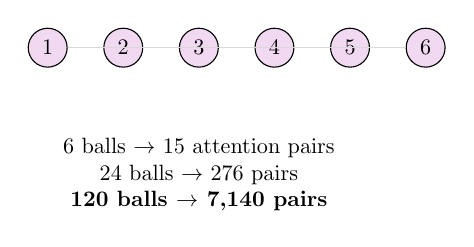
\begin{tikzpicture}[
    ball/.style={circle, draw, fill=ballcolor!40, minimum size=0.6cm},
    scale=0.8, transform shape
]
    % Balls
    \foreach \i in {1,...,6} {
        \node[ball] (b\i) at (\i*1.2, 0) {\i};
    }

    % All-to-all attention
    \foreach \i in {1,...,6} {
        \foreach \j in {1,...,6} {
            \ifnum\i<\j
                \draw[gray!30, thin] (b\i) -- (b\j);
            \fi
        }
    }

    \node[below=1cm of b3, align=center] {
        6 balls $\to$ 15 attention pairs\\
        24 balls $\to$ 276 pairs\\
        \textbf{120 balls $\to$ 7,140 pairs}
    };
\end{tikzpicture}
\caption{V1: Full attention scales O(n²)}
\end{figure}

\subsection{The Linear Solution (V2)}

In V2's graph, attention only flows along edges:

\begin{figure}[H]
\centering
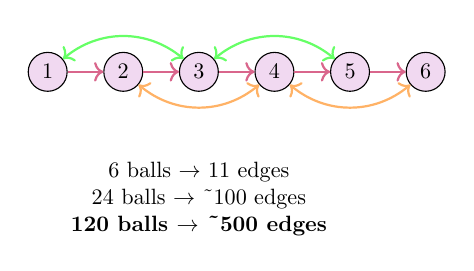
\begin{tikzpicture}[
    ball/.style={circle, draw, fill=ballcolor!40, minimum size=0.6cm},
    scale=0.8, transform shape
]
    % Balls (bowler A = 1,3,5 | bowler B = 2,4,6)
    \foreach \i in {1,...,6} {
        \node[ball] (b\i) at (\i*1.2, 0) {\i};
    }

    % Temporal edges only
    \foreach \i in {1,...,5} {
        \pgfmathtruncatemacro{\j}{\i+1}
        \draw[->, purple!60, thick] (b\i) -- (b\j);
    }

    % Same bowler (1-3-5)
    \draw[<->, green!60, thick, bend left=40] (b1) to (b3);
    \draw[<->, green!60, thick, bend left=40] (b3) to (b5);

    % Same bowler (2-4-6)
    \draw[<->, orange!60, thick, bend right=40] (b2) to (b4);
    \draw[<->, orange!60, thick, bend right=40] (b4) to (b6);

    \node[below=1cm of b3, align=center] {
        6 balls $\to$ 11 edges\\
        24 balls $\to$ \textasciitilde100 edges\\
        \textbf{120 balls $\to$ \textasciitilde500 edges}
    };
\end{tikzpicture}
\caption{V2: Sparse edges scale O(n)}
\end{figure}

\subsection{Efficiency Comparison}

\begin{table}[H]
\centering
\begin{tabular}{lccc}
\toprule
History Length & V1 Attention Pairs & V2 Edges & Speedup \\
\midrule
24 balls & 576 & \textasciitilde150 & 4x \\
60 balls & 3,600 & \textasciitilde350 & 10x \\
120 balls (full innings) & 14,400 & \textasciitilde700 & \textbf{20x} \\
\bottomrule
\end{tabular}
\caption{Computational comparison: V1 vs V2}
\end{table}

\newpage
%==========================================
\section{Model Architecture}
%==========================================

\subsection{Three-Stage Pipeline}

\begin{figure}[H]
\centering
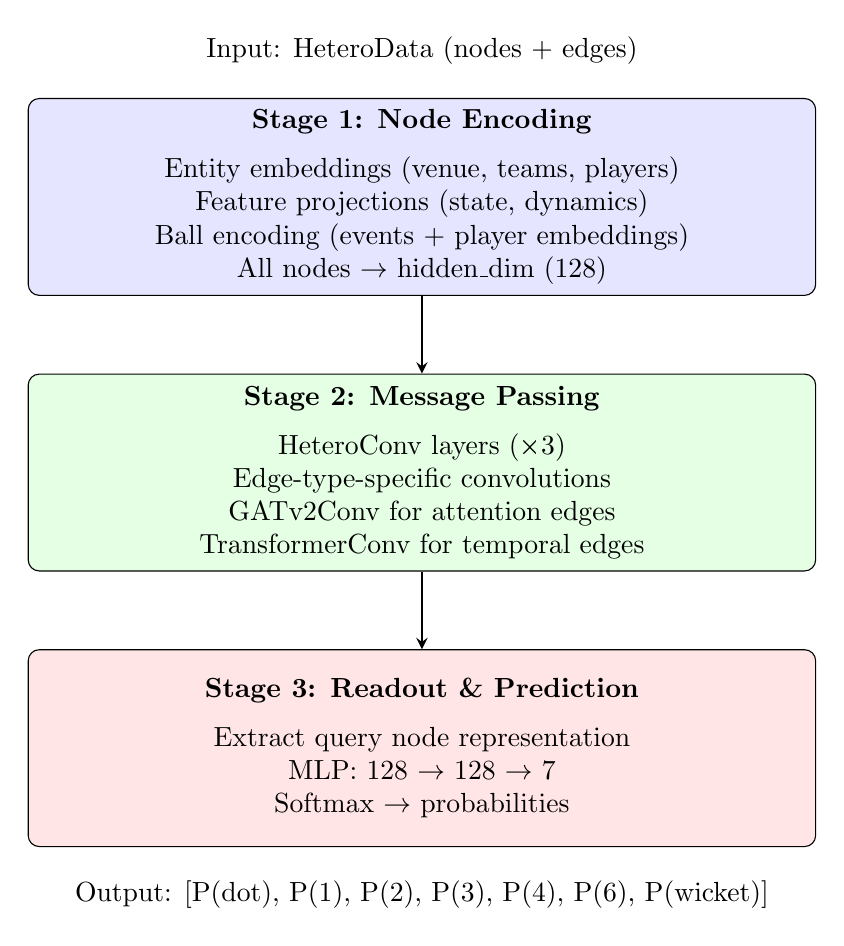
\begin{tikzpicture}[
    stage/.style={rectangle, draw, rounded corners, minimum width=10cm, minimum height=2.5cm, align=center},
    arrow/.style={->, thick, >=stealth}
]
    % Stage 1
    \node[stage, fill=blue!10] (s1) at (0, 6) {
        \textbf{Stage 1: Node Encoding}\\[0.2cm]
        Entity embeddings (venue, teams, players)\\
        Feature projections (state, dynamics)\\
        Ball encoding (events + player embeddings)\\
        All nodes $\to$ hidden\_dim (128)
    };

    % Stage 2
    \node[stage, fill=green!10] (s2) at (0, 2.5) {
        \textbf{Stage 2: Message Passing}\\[0.2cm]
        HeteroConv layers (×3)\\
        Edge-type-specific convolutions\\
        GATv2Conv for attention edges\\
        TransformerConv for temporal edges
    };

    % Stage 3
    \node[stage, fill=red!10] (s3) at (0, -1) {
        \textbf{Stage 3: Readout \& Prediction}\\[0.2cm]
        Extract query node representation\\
        MLP: 128 $\to$ 128 $\to$ 7\\
        Softmax $\to$ probabilities
    };

    \draw[arrow] (s1) -- (s2);
    \draw[arrow] (s2) -- (s3);

    % Input/Output
    \node[above=0.3cm of s1] {Input: HeteroData (nodes + edges)};
    \node[below=0.3cm of s3] {Output: [P(dot), P(1), P(2), P(3), P(4), P(6), P(wicket)]};
\end{tikzpicture}
\caption{Three-stage model pipeline}
\end{figure}

\subsection{Convolution Choices per Edge Type}

\begin{table}[H]
\centering
\begin{tabular}{lll}
\toprule
Edge Type & Convolution & Rationale \\
\midrule
Hierarchical & GATv2Conv & Attention learns which context matters \\
Intra-layer & GATv2Conv & Self-attention for permutation equivariance \\
Actor matchup & GATv2Conv & Learn matchup dynamics \\
Temporal (precedes) & TransformerConv & Edge features for temporal distance \\
Same-bowler/batsman & GATv2Conv & Aggregate spell patterns \\
Cross-domain & SAGEConv & Simple aggregation \\
Query & GATv2Conv & Learn what to attend for prediction \\
\bottomrule
\end{tabular}
\caption{Edge-type-specific convolution operators}
\end{table}

\newpage
%==========================================
\section{Temporal Edge Structure}
%==========================================

\subsection{Three Types of Ball-to-Ball Edges}

\begin{figure}[H]
\centering
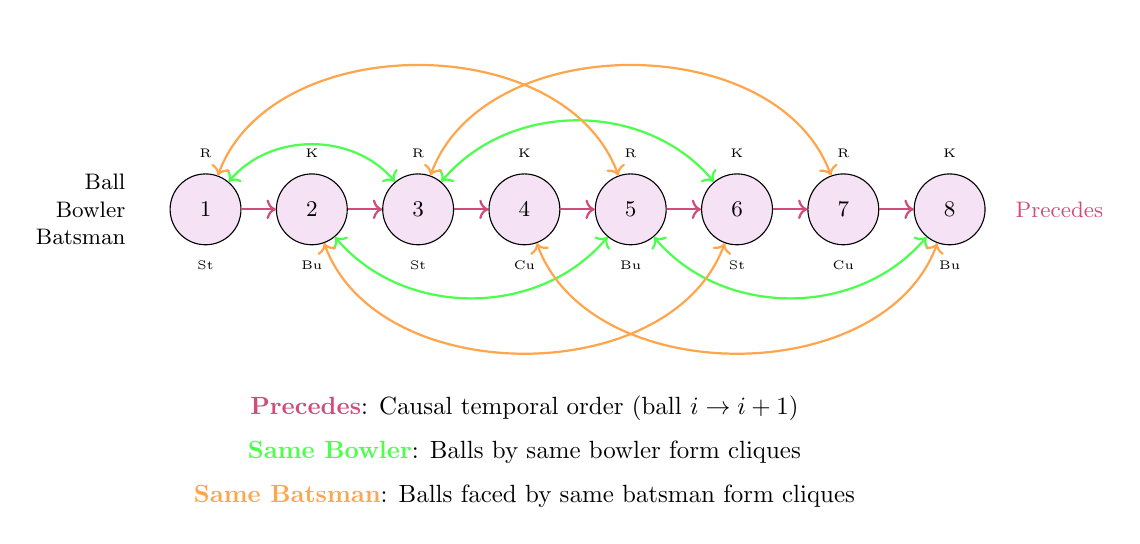
\begin{tikzpicture}[
    ball/.style={circle, draw, minimum size=1cm, font=\small},
    scale=0.9, transform shape
]
    % Row of balls
    \foreach \i/\b/\ba in {1/St/R, 2/Bu/K, 3/St/R, 4/Cu/K, 5/Bu/R, 6/St/K, 7/Cu/R, 8/Bu/K} {
        \node[ball, fill=ballcolor!30] (b\i) at (\i*1.5, 0) {\i};
        \node[below=0.1cm of b\i, font=\tiny] {\b};
        \node[above=0.1cm of b\i, font=\tiny] {\ba};
    }

    % Legend
    \node[left=0.5cm of b1, align=right, font=\small] {Ball\\Bowler\\Batsman};

    % Temporal edges
    \foreach \i in {1,...,7} {
        \pgfmathtruncatemacro{\j}{\i+1}
        \draw[->, thick, purple!70] (b\i) -- (b\j);
    }
    \node[right=0.3cm of b8, font=\small, purple!70] {Precedes};

    % Same bowler: Starc (1,3,6)
    \draw[<->, thick, green!70, bend left=50] (b1) to (b3);
    \draw[<->, thick, green!70, bend left=50] (b3) to (b6);

    % Same bowler: Bumrah (2,5,8)
    \draw[<->, thick, green!70, bend right=50] (b2) to (b5);
    \draw[<->, thick, green!70, bend right=50] (b5) to (b8);

    % Same batsman: Rohit (1,3,5,7)
    \draw[<->, thick, orange!70, bend left=70] (b1) to (b5);
    \draw[<->, thick, orange!70, bend left=70] (b3) to (b7);

    % Same batsman: Kohli (2,4,6,8)
    \draw[<->, thick, orange!70, bend right=70] (b2) to (b6);
    \draw[<->, thick, orange!70, bend right=70] (b4) to (b8);

    % Labels
    \node[below=2cm of b4, align=center] {
        \textcolor{purple!70}{\textbf{Precedes}}: Causal temporal order (ball $i \to i+1$)\\[0.2cm]
        \textcolor{green!70}{\textbf{Same Bowler}}: Balls by same bowler form cliques\\[0.2cm]
        \textcolor{orange!70}{\textbf{Same Batsman}}: Balls faced by same batsman form cliques
    };
\end{tikzpicture}
\caption{Temporal edge structure enables efficient pattern learning}
\end{figure}

\subsection{Why This Structure Matters}

\begin{itemize}
    \item \textbf{Precedes}: Captures immediate context, momentum shifts
    \item \textbf{Same Bowler}: How is this bowler's spell going? Patterns in their deliveries
    \item \textbf{Same Batsman}: How is this batsman building their innings?
\end{itemize}

In V1, these patterns were captured via soft attention biases.\\
In V2, they are \textbf{explicit graph structure} that the model must respect.

\newpage
%==========================================
\section{The Actor Matchup Graph}
%==========================================

\begin{figure}[H]
\centering
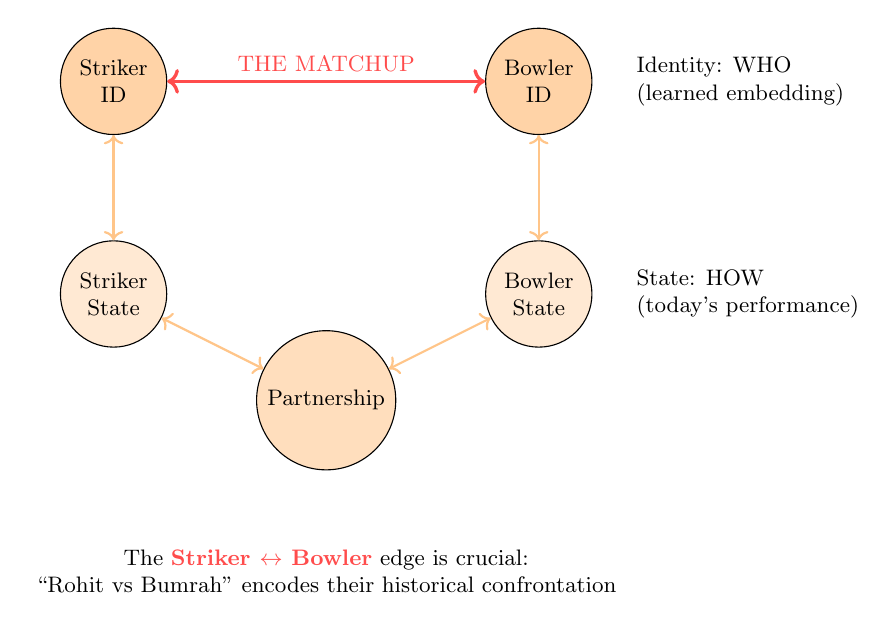
\begin{tikzpicture}[
    identity/.style={circle, draw, fill=actorcolor!60, minimum size=1.5cm, align=center, font=\small},
    state/.style={circle, draw, fill=actorcolor!30, minimum size=1.5cm, align=center, font=\small},
    partnership/.style={circle, draw, fill=actorcolor!45, minimum size=1.5cm, align=center, font=\small},
    edge/.style={<->, thick},
    scale=0.9, transform shape
]
    % Striker side
    \node[identity] (si) at (-3, 2) {Striker\\ID};
    \node[state] (ss) at (-3, -1) {Striker\\State};

    % Bowler side
    \node[identity] (bi) at (3, 2) {Bowler\\ID};
    \node[state] (bs) at (3, -1) {Bowler\\State};

    % Partnership
    \node[partnership] (p) at (0, -2.5) {Partnership};

    % Edges
    \draw[edge, actorcolor!80] (si) -- (ss);
    \draw[edge, actorcolor!80] (bi) -- (bs);
    \draw[edge, red!70, very thick] (si) -- node[above, font=\small] {THE MATCHUP} (bi);
    \draw[edge, actorcolor!80] (ss) -- (p);
    \draw[edge, actorcolor!80] (bs) -- (p);

    % Annotations
    \node[right=0.5cm of bi, align=left, font=\small] {
        Identity: WHO\\
        (learned embedding)
    };
    \node[right=0.5cm of bs, align=left, font=\small] {
        State: HOW\\
        (today's performance)
    };

    % Key insight
    \node[below=1cm of p, align=center, font=\small] {
        The \textcolor{red!70}{\textbf{Striker $\leftrightarrow$ Bowler}} edge is crucial:\\
        ``Rohit vs Bumrah'' encodes their historical confrontation
    };
\end{tikzpicture}
\caption{Actor layer graph structure (same as V1, now explicit)}
\end{figure}

%==========================================
\section{Data Flow Summary}
%==========================================

\begin{figure}[H]
\centering
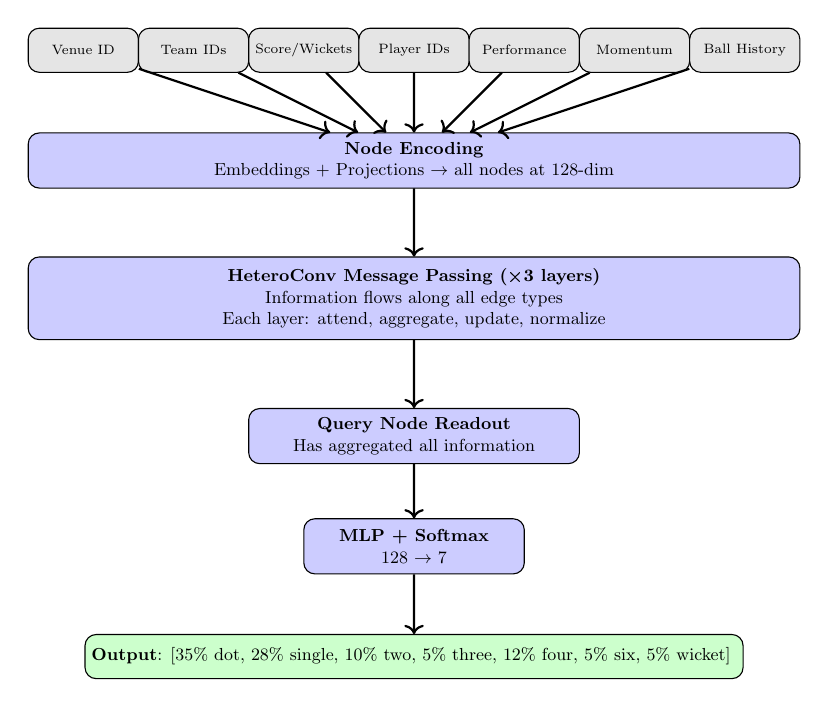
\begin{tikzpicture}[
    input/.style={rectangle, draw, rounded corners, fill=gray!20, minimum width=2cm, minimum height=0.8cm, align=center, font=\scriptsize},
    proc/.style={rectangle, draw, rounded corners, fill=blue!20, minimum width=3cm, minimum height=1cm, align=center, font=\small},
    output/.style={rectangle, draw, rounded corners, fill=green!20, minimum width=2.5cm, minimum height=0.8cm, align=center, font=\small},
    scale=0.7, transform shape
]
    % Raw inputs
    \node[input] (venue) at (-6, 8) {Venue ID};
    \node[input] (teams) at (-4, 8) {Team IDs};
    \node[input] (score) at (-2, 8) {Score/Wickets};
    \node[input] (players) at (0, 8) {Player IDs};
    \node[input] (perf) at (2, 8) {Performance};
    \node[input] (mom) at (4, 8) {Momentum};
    \node[input] (balls) at (6, 8) {Ball History};

    % Encoding
    \node[proc, minimum width=14cm] (encode) at (0, 6) {
        \textbf{Node Encoding}\\
        Embeddings + Projections $\to$ all nodes at 128-dim
    };

    % Message passing
    \node[proc, minimum width=14cm, minimum height=1.5cm] (mp) at (0, 3.5) {
        \textbf{HeteroConv Message Passing (×3 layers)}\\
        Information flows along all edge types\\
        Each layer: attend, aggregate, update, normalize
    };

    % Query
    \node[proc, minimum width=6cm] (query) at (0, 1) {
        \textbf{Query Node Readout}\\
        Has aggregated all information
    };

    % Prediction
    \node[proc, minimum width=4cm] (pred) at (0, -1) {
        \textbf{MLP + Softmax}\\
        128 $\to$ 7
    };

    % Output
    \node[output, minimum width=10cm] (out) at (0, -3) {
        \textbf{Output}: [35\% dot, 28\% single, 10\% two, 5\% three, 12\% four, 5\% six, 5\% wicket]
    };

    % Arrows
    \foreach \n in {venue, teams, score, players, perf, mom, balls} {
        \draw[->, thick] (\n) -- (encode);
    }
    \draw[->, thick] (encode) -- (mp);
    \draw[->, thick] (mp) -- (query);
    \draw[->, thick] (query) -- (pred);
    \draw[->, thick] (pred) -- (out);
\end{tikzpicture}
\caption{Complete data flow from raw inputs to prediction}
\end{figure}

\newpage
%==========================================
\section{Implementation Summary}
%==========================================

\subsection{Key PyTorch Geometric Components}

\begin{table}[H]
\centering
\begin{tabular}{ll}
\toprule
Component & PyG Class \\
\midrule
Data structure & \texttt{HeteroData} \\
Message passing & \texttt{HeteroConv} \\
Attention convolution & \texttt{GATv2Conv} \\
Temporal convolution & \texttt{TransformerConv} \\
Simple aggregation & \texttt{SAGEConv} \\
Batching & \texttt{DataLoader} (auto-batches HeteroData) \\
\bottomrule
\end{tabular}
\end{table}

\subsection{Model Configuration}

\begin{table}[H]
\centering
\begin{tabular}{lc}
\toprule
Parameter & Value \\
\midrule
Hidden dimension & 128 \\
Number of layers & 3 \\
Attention heads & 4 \\
Dropout & 0.1 \\
Number of classes & 7 \\
\midrule
Estimated parameters & \textasciitilde720K \\
\bottomrule
\end{tabular}
\end{table}

\subsection{Training Details}

\begin{itemize}
    \item \textbf{Loss}: Cross-entropy with class weights (imbalanced outcomes)
    \item \textbf{Optimizer}: AdamW (lr=1e-3, weight\_decay=0.01)
    \item \textbf{Scheduler}: Cosine annealing
    \item \textbf{Early stopping}: Patience of 10 epochs
\end{itemize}

%==========================================
\section{Interpretability Benefits}
%==========================================

The unified graph provides natural interpretability:

\begin{enumerate}
    \item \textbf{Edge attention weights}: Which historical balls mattered most?
    \item \textbf{Same-bowler attention}: How much did the bowler's spell inform the prediction?
    \item \textbf{Matchup attention}: How important was the striker-bowler confrontation?
    \item \textbf{Hierarchical attention}: Did global context (venue) or local dynamics drive the prediction?
\end{enumerate}

All of these are directly extractable from the GATv2Conv attention weights.

\end{document}
